\documentclass[conference]{IEEEtran}
% \IEEEoverridecommandlockouts
% The preceding line is only needed to identify funding in the first footnote. If that is unneeded, please comment it out.
\usepackage{cite}
\usepackage{amsmath,amssymb,amsfonts}
\usepackage{algorithmic}
\usepackage{graphicx}
\usepackage{textcomp}
\usepackage{xcolor}
\def\BibTeX{{\rm B\kern-.05em{\sc i\kern-.025em b}\kern-.08em
    T\kern-.1667em\lower.7ex\hbox{E}\kern-.125emX}}
\begin{document}

\title{Application for Pseudocode Interpretation and Code Analysis}

\author{\IEEEauthorblockN{Lóránt Áron Perger}
\IEEEauthorblockA{\textit{John von Neumann Faculty of Informatics} \\
\textit{Óbuda University}\\
Budapest, Hungary \\
pergerlori@gmail.com}
\and
\IEEEauthorblockN{Ádám Pintér}
\IEEEauthorblockA{\textit{John von Neumann Faculty of Informatics} \\
\textit{Óbuda University}\\
Budapest, Hungary \\
pinter.adam@nik.uni-obuda.hu}
}

\maketitle

\begin{abstract}
The following paper describes the implementation of an application capable of interpreting and executing algorithms written in the Pszeudokód programming language taught at Óbuda University. The process is explained starting with the formalization of the language's rules from an informal specification, followed by the methods of transforming source code into an executable format, and concluded with showing the means of allowing students to look into the inner workings of the running code.
\end{abstract}

\begin{IEEEkeywords}
compiler, interpreter, parsing, tokenizing, ast, code analysis
\end{IEEEkeywords}

\section{Introduction}

During their first year at Óbuda University, students are introduced to an imaginary programming language called Pszeudokód ("pseudo-code"), which is a simplified, C/Pascal-like imperative language, created to teach the basics of programming and algorithmic thinking.

When I was first beginning my studies, the fact that this language only existed in print and did not have a compiler/interpreter really hindered my progress at understanding the algorithms, despite that I came to this university already knowing the basics of programming.

Because of this, I decided to pick the creation of such a program as the topic of my dissertation and project-work and thus make something that both allows me to explore the inner workings of a compiler and result in an application that could help subsequent students at successfully passing their course.

During the creation of this application, I first documented the process of creating a simple, formal specification of a language from the informal, mostly example-based lecture notes, which for the most part leaves the rules of the language to intuition. This was then followed the creation of a four-step compiler which takes input strings that adhere to this specification and constructs an array of instructions. I have then created a simple virtual machine that takes the previously created array and executes it in a way that allows the user to both glance into the inner workings of the algorithm and to be able to stop and step through it at arbitrary points.

\section{Related Work}

As it serves the very base of our field, the topic of programming languages is huge and diverse. Enumerating every programming language would be just as unfruitful as it is impossible.

Instead I would like to name a few languages and projects that allowed me to understand the process of implementing a compiler.

Firstly, I cannot leave out the famous *Structure and Interpretation of Programming Languages,* a book which was used at MIT to teach students programming in the Scheme language from the very basics, up to the level of writing an actual compiler for the same language. It was one of the biggest inspirations for my dissertation and it was the work that finally made me make the realization that ultimately compilers themselves are simply programs as well.

Secondly, I would like to name Robert Nystrom's *Crafting Interpreters,* which is an excellent, in-depth tutorial about creating a fairly elaborate programming language. This book's clear and succinct explanations gave me the idea of what the big steps of transformation should be in my own application.

Thirdly, Michael R. Clarkson's *OCaml Programming: Correct + Efficient + Beautiful* provided great help in comprehending the process of inferring and checking the types of our program, along with the idea of static environments (a map-type data-structure, which stores the names of variables and the values associated with these).

Finally, of course, I must also mention the lecture notes used at the university, as it serves the backbone of my entire dissertation. These notes define the overall syntax and structure of Pszeudokód, along with all of the algorithms contained in my program.

\section{Methodology}

Our goal is to turn the users' raw, source code into a format that can not only be executed, but also stepped through and paused at any given instruction. To accomplish this, we have to utilize a variety of simpler and more complex steps. These will be discussed separately below, but first I would like to present the complete plan of the program in figure \eqref{fig:system}.

\begin{figure}[htbp]
\centerline{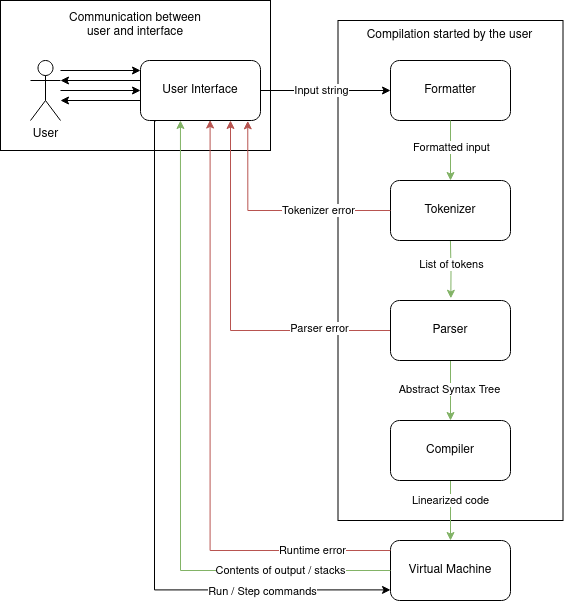
\includegraphics[width=0.45\textwidth]{rendszerterv_en.png}}
\caption{Visualization of the application's main stages}
\label{fig:system}
\end{figure}

\subsection{Specification}

Technically speaking this is not a step, as the work is purely theoretical. As the lecture notes do not rigidly set the rules of the language, this is something I had to do first before I could begin implementing my compiler.

I began by identifying the individual elements of the language, building up its rules and syntax, which are together called the *grammar* of a language. As Pszeudokód is an imperative language, I separated its elements into statements (instructions that control the program's flow) and expressions (instructions that calculate actual values) and also determined the three base types (numbers, strings, and boolean values).

I then presented the grammar in a notation called Extended Bachus-Naur Form, which allows the precise description of syntax, along with a textual listing of the rules of each element.

Finally, I also took note of the few places where I decided to deviate from the lecture notes' implied rules, as some of these only make sense in printed format or contain no useful information to the compiler.

\subsection{Formatting}

Though the process of compilation really begins here, the choice of including this step was entirely optional, as the program is entirely capable of processing inputs regardless of their whitespace (which is ignored by the language and only serves the separation of syntactical elements). However, because this program was created with a pedagogical goal in mind, I decided that providing a consistent coding style regardless of user input would allow students to focus more on the algorithm itself than how to structure it.

To this end, the formatter is an extremely simple algorithm that walks the source code broken into an array of lines. On each element, it calculates the new level of indentation from the previous line, utilizing information such as the previous line's indentation, whether the previous line was indented or dedented, and what the current line contains.

Though in a more sophisticated program, it would not be unreasonable to tokenize and parse the code first, then turn the resulting syntax tree back into well-formatted code, this method allows for a far simpler implementation, at the cost of less fine-tuned control over the formatting itself.

\subsection{Tokenization}

The process of tokenization is when the source code is split into the smallest individual elements (so-called "tokens"), which hold meaning in the language we are trying to interpret. Though strictly speaking this step too is optional, as there exist parsers, which build their trees directly from text, without any previous transformations, the inclusion of this step provides some strong benefits.

For one, it clearly separates two concerns in the code. Once we reach the step of parsing, we should not need to worry about the exact shape of the individual syntactical elements, just their presence. Thus this pre-processing step simplifies our code.

Secondly, and more importantly, it allows us to endow our tokens with extra information which might be used for error diagnostics and even convenience features like syntax highlighting, which my program implements.

The tokenizer is implemented using a simple left-to-right scan of the source code, during which we loop over the possible patterns, which may either be exact strings, such as keywords, parentheses, etc. or predicates, such as strings being a quote followed by an arbitrary amount of characters, followed by another quote. If we happen to find a matching pattern, we return a token with the appropriate type, the row and column of where the matching string starts, and finally the *lexeme,* which is the actual matched string. If the tokenizer cannot match any one of the possible patterns, we create a special token that denotes an error and immediately assign the rest of the input to it and quit the algorithm.

Regardless of whether we were successfully able to match the entire input or not, we're ultimately left with an array of tokens, which is then passed on to the next step.

\subsection{Parsing}

Given an array of tokens, a parser algorithm is capable of constructing a data-structure named *abstract syntax-tree* (AST), which is a hierarchical representation of the program's structure and control flow, that discards all information not strictly necessary for the interpretation of the program, such as comments and whitespace.

Generally parsers are implemented either as recursive-descent parsers, which work very similarly to the tokenizer algorithm described above or so-called Parser-Expression-Grammars (PEG), which are an extension of regular expressions. For me the former method felt too mechanical, as it requires manually implementing each and every case and its error handling, which can quickly grow beyond the point of maintainability. The latter method is even more complex and because of that, both are usually not written by hand these days, but rather using tools called parser-generators.

I, however, wanted to minimize the amount of external tools I have used to implement my application, as I did not want any of the steps involved to feel like a black box. Therefore, my implementation of the parsing algorithm is a manually written version of the monadic combinator parser method, adapted from a paper written for the Haskell programming language.

The base unit of parsing in this variant is the *combinator,* a function which, when given an input (usually consisting of either the raw source code string or a list of tokens and an index showing how far we've already parsed), produces a value of arbitrary type and a modified copy of the input, whose index is incremented by the amount of elements it had processed. Because of this latter property, it is very easy to chain these functions into each other and progressively build up more and more complex parsers, until we finally achieve one that is capable of parsing complete programs.

This chaining is done through a method called `bind`, which takes a parser and a function whose input is a value of the same type as the aforementioned parser's output type and outputs a new parser of arbitrary type. This way we can chain as many parsers into each other as we wish, while doing separate computations on their return values.

The paper defines common operators and building blocks, such as the `or` combinator, which takes two other combinators as input and return another combinator, that first tries the first input and if that fails, returns with the result of the second. Similar methods exist for executing a parser multiple times, parsing a list and throwing away the separator elements, parsing an element surrounded by brackets or quotes, etc.

Another benefit of this method is that if the process ever fails, we do not need to write any special code to handle the error path, as the way functions are chained together has short-circuiting built in. That is to say in case of parsing failure, the error is immediately bubbled through the rest of the function calls and becomes the final return value.

\subsection{Typechecking}

Provided we reach this point, our original input is guaranteed to be syntactically correct, meaning it only uses combinations of elements defined by the language's specification. However, such a program is not guaranteed to be semantically correct. A trivial example is attempting to do arithmetics on string type values, which generally leads to nonsensical results if not outright crashes.

To prevent such cases, we create an algorithm that is capable of reasoning about the program's control flow and the types of the individual values and variables present in the program. Using these, the algorithm checks whether our types are consistent, that is to say the programmer never attempts to do something that goes against the specified semantics.

This is done through a recursive-descent function, whose input is the currently checked node of the AST and a data-structure called a *type map,* which will be defined shortly. Using these two values, the algorithm checks if it had reached an atomic value (these are the language's base types, which need no further context or information to be meaningful, such as numbers, strings, or boolean values) and if so, returns with its type. If the node currently checked is not an atomic value, we recursively call the algorithm on its child nodes, while also making sure the language's rules are not broken.

In cases when we are dealing with variables and functions, whose types should remain unchanging and consistent through multiple instructions, we utilize the aforementioned type map, which is a data-structure capable of associating names with types. During every call of the recursive typechecking function, we pass forward a copy of the current type map, this way variables and functions will only be valid after they were declared and will become unavailable once we leave their scope.

As the language also supports generic functions, the type map is capable of storing and later substituting generic types for concrete ones. This is done by having a separate list in the data-structure, which we walk through whenever we encounter a type and check if said type contains anything we should substitute.

One might wonder why we are not simply checking whether the type itself is generic and substituting based on that fact and the reason is that in my implementation types are represented using nested classes, for instance an array of numbers would be `ArrayType(SimpleType(BaseType.NUMBER))` and thus if we were making a `T` generic array, we'd get `ArrayType(GenericType("T"))` and the previously mentioned simple comparison would return false, as it only sees that the type is an array variant.

\subsection{Linearization of code}

With the typechecking done, we can now be certain that our code is both syntactically and semantically correct. If our goal was merely to execute the input algorithm, this following step could be skipped. However, because a main goal of this application is to allow users to stop the execution at arbitrary points and step through the code, we need to do one more pre-processing pass.

This is what I call the *linearization of code,* as it takes a hierarchical syntax-tree and breaks it into a linear array of atomic operations ("atomic" here meaning that the individual instructions do not rely on each other and can be executed by themselves).

This is done with yet another recursive-descent walk of the tree, during which we visit the nodes in a pre-set order and emit so-called *bytecode* depending on what variant we have encountered.

This bytecode is a compact representation of what the runtime environment should do during each instruction. It is characterized by an "operation code" (opcode), a unique value associated with the kind of operation we intend to execute and an arbitrary amount of extra, compile-time information encoded as extra fields.

Because we assume that our code is correct at this point, this step does no further validation and any incorrect data results in the raising of an exception.

\subsection{Execution}

Once we have our linear bytecode, we are practically done with the compilation. The only step left is to have an environment that is capable of executing it.

This is accomplished through a simple, stack-based virtual machine (VM), that implements a tiny, custom architecture. The VM is loaded with the bytecode, which is then executed until either it reaches the end of the code or a `debug` instruction, that will immediately stop execution and allow the user to either continue running as previously or step through the code instruction-by-instruction.

To further facilitate helping the user understand the inner workings of the algorithm, the user interface driving the application is capable of showing the internal state of the VM, presenting the contents of its stack, the names of the variables and what values they were bound to, the contents of the memory, which line is currently being executed, and finally the call stack. This updates live as the user steps through code and highlights with colors whether a value was created (using green), changed (yellow) or deleted (red).

\section{Evaluation}

\subsection{Usability}

At the time of writing the compiler was tested to be capable of typechecking all ninety-six algorithms found in the lecture notes used by students during the first semester and is capable of executing the majority of them flawlessly. A handful of algorithms were also hand fed with inputs and compared with the expected output to make sure the VM is correctly executing the code. The process of this can be seen on figure \eqref{fig:testing}.

\begin{figure}[htbp]
\centerline{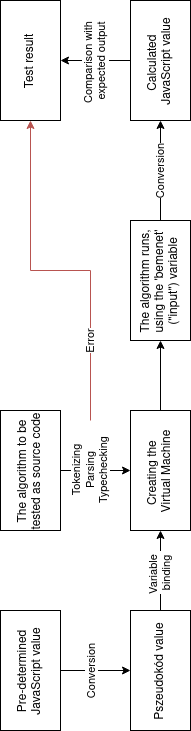
\includegraphics[height=0.6\textheight]{teszt_en2.png}}
\caption{Automated testing based on pre-determined input and output values}
\label{fig:testing}
\end{figure}

However, I was unable to implement some features of the language, which requires adapting the algorithms that use these to be able to be run through the application. One of these features is the fact that Pszeudokód stipulates that its equivalent of for-loops should be able to count both up and down using the same syntax. As the direction is not decidable during compilation (the two values between which we loop can be variables for instance), handling this edge-case would require a separate instruction in the virtual machine, which I considered excessive as an equivalent transformation of the code works without issue.

Similarly, I haven't implemented built-in support for some of the more exotic data-structures used by the language, such as sets and time-related primitives, as both of these are either given native algorithms or are so infrequently used that I could not justify the extra development time they would have taken.

\subsection{Performance}

The individual steps of the process was not measured, as performance was not a primary concern during development. To provide a rough estimate, the application did not show noticeable slowdowns throughout its testing, except for one area, which was the rendering of the VM's inner state. This was remedied by forbidding the application from re-rendering its user interface until the VM had stopped running. This has virtually eliminated all slowdowns of the program.

\section{Conclusions}

Besides the shortcomings described above, the final application fulfills the main goals set out by the paper. It is capable of interpreting valid Pszeudokód source code, while validating its syntactical and type correctness. It is also able to give useful information about the internal state of the application. Furthermore, the code is written in a way that allows for the addition of additional features and syntax in the hypothetical case that the compiler needs to be expanded to enable running algorithms found in the second semester lecture notes.


\end{document}
